\chapter{АПРОБАЦИЯ И АНАЛИЗ РЕЗУЛЬТАТОВ}
\label{ch:approbation}

\section{Цели, стенд и границы апробации}

Цель апробации состоит в проверке того, что разработанная платформа обеспечивает корректную фиксацию событий, соблюдение ролевой модели доступа и надежную доставку сведений о событиях при отказах интеграционного контура. Методика согласована с критериями, сформулированными в главах~\ref{ch:problem_statement} и~\ref{ch:model_algorithm}, а также с общей логикой испытаний интеллектуальной видеоаналитики в системах видеонаблюдения~\cite{iec_62676_4_2025,iec_62676_6_2026}.

Фактическая апробация выполнена в двух контурах:
\begin{enumerate}
    \item автоматизированный приемочный прогон на CPU-профиле стенда Docker Compose;
    \item демонстрационный профиль обнаружения БПЛА на заранее подготовленном видеофрагменте и обученных весах детектора.
\end{enumerate}

Аппаратное ускорение и многокамерная нагрузка рассматриваются как направление дальнейшего развития. В настоящей редакции количественные результаты заявляются только для CPU-профиля приемки и надежной доставки событий, а демонстрационный БПЛА-сценарий используется для проверки связности видеоконтура, операторского интерфейса и журнала событий.

Для исключения завышения выводов в работе используются три уровня доказательности. Первый уровень -- автоматизированный приемочный прогон \texttt{RUN-2026-05-13-A1}; по нему формулируются количественные значения задержек восстановления, статусов доставки и результатов RBAC-проверок. Второй уровень -- демонстрационный видеосценарий БПЛА; он подтверждает включение обученной модели в платформу и прохождение результата до интерфейса, но не используется как статистическая оценка промышленной задержки. Третий уровень -- расчетные критерии для будущего многокамерного стенда; они задают методику дальнейших измерений, но не объявляются достигнутым результатом настоящей апробации. В таблицах главы слово «пройден» относится только к явно указанному контуру проверки.

\begin{table}[H]
\caption{Контуры апробации и использованные артефакты}
\label{tab:approbation_profiles}
\begin{tabularx}{\textwidth}{>{\raggedright\arraybackslash}p{0.23\textwidth}>{\raggedright\arraybackslash}p{0.21\textwidth}>{\raggedright\arraybackslash}X}
\toprule
Контур & Артефакт & Назначение \\
\midrule
CPU-профиль приемки & JSON RUN-A1 & Проверка интеграционной доставки, RBAC, отказов RabbitMQ и HTTP-получателя \\
БПЛА-профиль & видео БПЛА и \texttt{best.pt} & Демонстрация обнаружения БПЛА и прохождения события через платформу \\
Обучение YOLO-детектора & \texttt{results.csv}, графики и матрица ошибок & Фиксация качества предметно дообученного детектора \\
План масштабирования & приложение В & Направление дальнейшего развития без заявленных приемочных метрик \\
\bottomrule
\end{tabularx}
\end{table}

\section{Экспериментальные данные и артефакты}

Для демонстрационного БПЛА-профиля использован набор данных Small Detection в формате YOLO с двумя целевыми классами: \texttt{bird} и \texttt{drone}. Этот профиль является отдельной конфигурацией целевых классов и не противоречит базовому охранному профилю с классами \texttt{person} и \texttt{vehicle}, описанному в главе~\ref{ch:model_algorithm}. Наличие специализированных наборов данных и слабоконтролируемых сценариев разметки важно именно для БПЛА-задач, поскольку объект часто занимает малую площадь кадра, меняет масштаб и наблюдается на неоднородном фоне~\cite{chen2026uavdb}.

\begin{table}[H]
\caption{Параметры набора данных и обучения детектора}
\label{tab:yolo_training_config}
\begin{tabularx}{\textwidth}{>{\raggedright\arraybackslash}p{0.32\textwidth}>{\raggedright\arraybackslash}X}
\toprule
Параметр & Значение \\
\midrule
Классы & \texttt{bird}, \texttt{drone} \\
Обучающая выборка & 3982 изображения \\
Валидационная выборка & 973 изображения \\
Базовая модель & вариант \texttt{yolo26n}, файл начальных весов \texttt{yolo26n.pt} \\
Размер входа & 640 пикселей \\
Число эпох & 100 \\
Размер пакета & 16 \\
Устройство обучения & Apple MPS \\
Итоговые веса & \texttt{best.pt} из каталога обучения \texttt{small\_detection} \\
\bottomrule
\end{tabularx}
\end{table}

К финальной эпохе обучения достигнуты следующие валидационные показатели: precision \(=0.8865\), recall \(=0.8677\), \(mAP_{50}=0.8810\), \(mAP_{50:95}=0.4161\). Значения взяты из последней строки файла \texttt{results.csv}; график обучения и матрица ошибок используются для визуального контроля динамики обучения и распределения ошибок. Эти значения не трактуются как промышленная сертификация детектора, но подтверждают пригодность модели для демонстрационного контура и дальнейшего дообучения на объектовых сценах.

\begin{figure}[H]
\centering

\includegraphics[width=0.95\textwidth]{yolo_training_results.png}
\caption{Динамика метрик обучения детектора YOLO}
\label{fig:yolo_training_results}
\end{figure}

\begin{figure}[H]
\centering

\includegraphics[width=0.74\textwidth]{yolo_confusion_matrix.png}
\caption{Матрица ошибок детектора на валидационной выборке}
\label{fig:yolo_confusion_matrix}
\end{figure}

Пример обнаружения БПЛА на демонстрационном видео приведен на рисунке~\ref{fig:drone_demo_detection}. Данный артефакт включен в отчет не как отдельное сравнительное испытание, а как проверка связности прикладного сценария: обученные веса подключены к \texttt{analytics-worker}, а результат используется для формирования событийного потока платформы.

\begin{figure}[H]
\centering
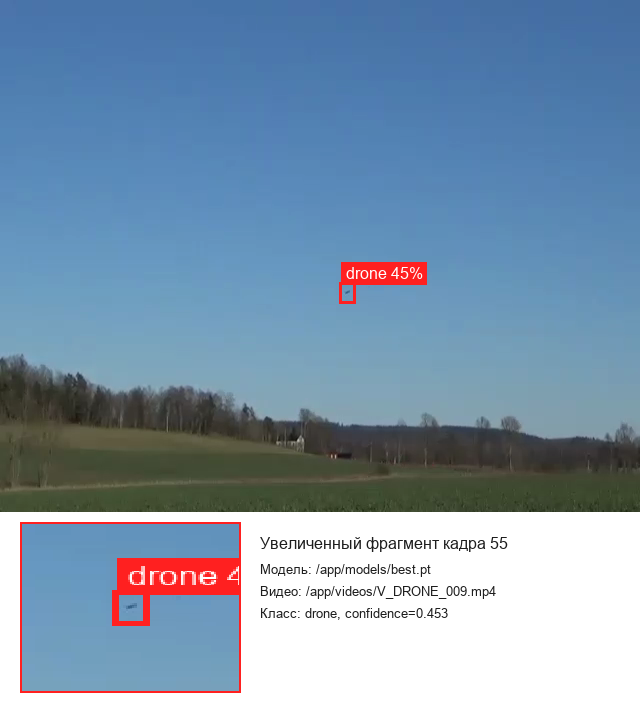
\includegraphics[width=0.72\textwidth]{drone_demo_detection.png}
\caption{Пример обнаружения БПЛА в демонстрационном видеофрагменте}
\label{fig:drone_demo_detection}
\end{figure}

\section{Метрики и порядок расчета}

Пусть \(\Delta t_j\) -- задержка от фиксации факта появления объекта до записи соответствующего события в таблицу исходящих сообщений для события \(j\). Тогда расчетная p95-оценка для серии прогонов задается выражением
\begin{equation}
\operatorname{p95}_{\text{obj}\to\text{event}} =
\operatorname{quantile}_{0.95}\{\Delta t_j\}.
\end{equation}

Доля отброшенных кадров:
\begin{equation}
R_{\text{drop}} = \frac{N_{\text{dropped}}}{N_{\text{input}}}.
\end{equation}

Доля успешной доставки во внешний контур:
\begin{equation}
R_{\text{delivery}} = \frac{N_{\text{delivered}}}{N_{\text{generated}}}.
\end{equation}

Для отказных сценариев дополнительно фиксируются:
\begin{itemize}
    \item статус записи исходящего сообщения во время отказа и после восстановления;
    \item число повторных попыток;
    \item количество успешных и неуспешных попыток доставки;
    \item время восстановления доставки после возврата внешнего компонента.
\end{itemize}

Для сценариев проверки безопасности критерием является соответствие фактического HTTP-статуса ожидаемому: например, попытка роли \texttt{viewer} выполнить операцию записи должна завершаться кодом 403.

Приемочный прогон считается успешным только при одновременном выполнении следующих условий: итоговое поле \texttt{result} в JSON-артефакте равно \texttt{passed}; запись исходящего сообщения для функционального сценария имеет статус \texttt{published}; счетчик успешных доставок функционального события равен единице при нулевом числе неуспешных доставок; при отказе RabbitMQ запись переходит в состояние \texttt{retry} и после восстановления получает статус \texttt{published}; при временной недоступности HTTP-получателя фиксируются неуспешные попытки и последующая успешная доставка; роль \texttt{viewer} получает запрет 403 при попытке выполнить операцию записи. Эти критерии проверяют не только наличие события, но и состояние транзакционной таблицы исходящих сообщений, транспортного контура и политики доступа.

\section{Результаты приемочного прогона}

Сохраненный приемочный артефакт \texttt{acceptance\_results\_2026-05-13.json} содержит результат \texttt{passed}; длительность автоматизированного прогона составила \(30.732\)~с. В рамках сценария были созданы тестовые сущности камеры, зоны и правила, после чего проверены прохождение синтетически зафиксированного события \texttt{zone\_enter} через интеграционный контур, отказ RabbitMQ, восстановление HTTP-получателя и запрет операции записи для роли \texttt{viewer}. Для событий \texttt{zone\_enter}, \texttt{line\_cross} и \texttt{dwell\_time} в данном прогоне проверялся не полный путь от видеокадра, а путь от записи события в базе данных до доставки внешнему HTTP-получателю.

Доказательная база приемочного прогона включает не только итоговый статус, но и контрольные поля артефакта: идентификаторы созданных камеры, зоны и правила; статусы записей таблицы исходящих сообщений до и после восстановления RabbitMQ; счетчики успешных и неуспешных доставок; время восстановления доставки; HTTP-статус 403 для запрещенной операции роли \texttt{viewer}. Таблицы ниже повторяют значения из JSON-артефакта и протоколов испытаний; они не являются самостоятельным источником измерений. Тем самым результат апробации связан с наблюдаемыми состояниями системы, а не с ручной оценкой интерфейса.

\begin{table}[H]
\caption{Функциональные результаты интеграционной проверки}
\label{tab:e2e_results}
\begin{tabularx}{\textwidth}{@{}>{\raggedright\arraybackslash}p{0.22\textwidth}>{\raggedright\arraybackslash}p{0.13\textwidth}>{\raggedright\arraybackslash}p{0.13\textwidth}>{\raggedright\arraybackslash}X@{}}
\toprule
Сценарий & Статус & Значение & Комментарий \\
\midrule
\texttt{zone\_enter} & пройден & 1 событие & Синтетическое событие зафиксировано, запись исходящего сообщения переведена в \texttt{published} \\
\texttt{line\_cross} & пройден & синт. событие & Проверен проход через таблицу исходящих сообщений и интеграционный контур \\
\texttt{dwell\_time} & пройден & синт. событие & Проверен проход через контур повторной доставки HTTP-получателю \\
Интеграционная доставка & пройдена & success \(=1\), failed \(=0\) & Базовое событие доставлено внешнему HTTP-получателю \\
\bottomrule
\end{tabularx}
\end{table}

\begin{table}[H]
\caption{Проверка надежности доставки при отказах}
\label{tab:reliability_results}
\begin{tabularx}{\textwidth}{>{\raggedright\arraybackslash}p{0.26\textwidth}>{\raggedright\arraybackslash}p{0.17\textwidth}>{\raggedright\arraybackslash}p{0.18\textwidth}>{\raggedright\arraybackslash}X}
\toprule
Сценарий & Потери & Время восстановления & Комментарий \\
\midrule
Отказ RabbitMQ & 0 & \(8.863\)~с & Во время отказа запись исходящего сообщения имела статус \texttt{retry}; после восстановления статус стал \texttt{published} \\
Недоступность HTTP-получателя & 0 & \(4.455\)~с & Зафиксированы неуспешные попытки, затем успешная доставка после восстановления \texttt{webhook-mock} \\
Очередь недоставленных сообщений при исчерпании повторов & нет данных RUN-A1 & не измерялось & Переход в очередь недоставленных сообщений проверен отдельным тестом логики фонового обработчика; длительная недоступность HTTP-получателя требует отдельного стендового прогона \\
\bottomrule
\end{tabularx}
\end{table}

\begin{table}[H]
\caption{Результаты проверки безопасности в приемочном прогоне}
\label{tab:security_results}
\begin{tabularx}{\textwidth}{>{\raggedright\arraybackslash}p{0.34\textwidth}>{\raggedright\arraybackslash}p{0.18\textwidth}>{\raggedright\arraybackslash}X}
\toprule
Проверка & Результат & Интерпретация \\
\midrule
Вход администратора & пройден & Маркеры доступа и обновления выданы, профиль роли доступен \\
\texttt{viewer} создает камеру & 403 & Запрет операции записи соответствует RBAC-матрице \\
Обновление и завершение сессии & пройден & Маркер обновления отзывается, повторное обновление запрещено \\
Валидация зон и правил & пройдена & Некорректные параметры полигона, линии и длительности отклоняются API \\
\bottomrule
\end{tabularx}
\end{table}

\begin{table}[H]
\caption{Производительность и эксплуатационные показатели}
\label{tab:perf_results}
\begin{tabularx}{\textwidth}{>{\raggedright\arraybackslash}p{0.3\textwidth}>{\raggedright\arraybackslash}p{0.22\textwidth}>{\raggedright\arraybackslash}X}
\toprule
Показатель & Значение & Комментарий \\
\midrule
Длительность приемочного прогона & \(30.732\)~с & Автоматизированный функционально-отказной прогон \\
Задержка функциональной доставки & \(4.605\)~с & Одиночное измерение интеграционной доставки; для p95 полного видеоконтура нужна серия длительных прогонов \\
Задержка восстановления RabbitMQ & \(8.863\)~с & Время до публикации после восстановления брокера \\
Задержка восстановления HTTP-получателя & \(4.455\)~с & Время до успешной доставки после восстановления HTTP-получателя \\
Число сообщений в очереди недоставленных & 0 в RUN-A1 & В штатном приемочном прогоне сообщений в очереди недоставленных не зафиксировано; сценарий исчерпания повторов проверен отдельно на уровне логики фонового обработчика \\
YOLO \(mAP_{50}\) & \(0.8810\) & Метрика автономной валидации демонстрационного детектора \\
\bottomrule
\end{tabularx}
\end{table}

\section{Интерпретация результатов}

Полученные результаты подтверждают достижение ключевых инженерных свойств платформы:
\begin{itemize}
    \item функциональная цепочка «событие -- таблица исходящих сообщений -- RabbitMQ -- HTTP-получатель» работает для проверенных синтетически зафиксированных событий;
    \item кратковременная недоступность RabbitMQ не приводит к потере событий, так как факт события сохраняется в БД до восстановления публикации;
    \item недоступность HTTP-получателя приводит к контролируемым неуспешным попыткам и последующей успешной доставке после восстановления;
    \item роль \texttt{viewer} не может изменять конфигурацию камер, что подтверждает применимость RBAC-политики для базового контура безопасности;
    \item предметно дообученный детектор демонстрирует достаточные автономно измеренные показатели для включения в демонстрационный контур БПЛА.
\end{itemize}

Вместе с тем количественная оценка p95 \(\texttt{object}\rightarrow\texttt{event}\) требует не одиночного приемочного прогона, а серии длительных измерений при фиксированном числе камер, одинаковой частоте кадров и сохраненных временных рядах. Поэтому в настоящей работе p95-критерий оставлен как формальный приемочный критерий, а не как заявленное промышленное значение для всех профилей.

\section{Ограничения апробации и угрозы валидности}

\begin{table}[H]
\caption{Ограничения экспериментов и меры снижения риска}
\label{tab:validity_threats}
\begin{tabularx}{\textwidth}{>{\raggedright\arraybackslash}p{0.27\textwidth}>{\raggedright\arraybackslash}X}
\toprule
Ограничение & Влияние и мера контроля \\
\midrule
Одиночный приемочный прогон & Позволяет проверить корректность сценариев, но не заменяет статистически устойчивую p95-оценку \\
Синтетические интеграционные события & Подтверждают путь доставки, но не измеряют полный вклад декодирования и инференса \\
Ограниченный набор БПЛА-сцен & Демонстрация требует расширения на реальные объектовые условия, разные фоны и масштабы \\
Нет длительной многокамерной серии & Не позволяет утверждать промышленные p95-границы; такие измерения вынесены в следующий стендовый этап \\
Очередь недоставленных сообщений не проверялась стендовым прогоном с исчерпанием повторов & Подтверждена логика перехода в очередь недоставленных сообщений, но не измерены длительность и операционные последствия длительного отказа HTTP-получателя \\
Односерверное развертывание & Проверяет базовую архитектуру, но не покрывает кластерную конфигурацию высокой доступности (HA) для PostgreSQL/RabbitMQ \\
\bottomrule
\end{tabularx}
\end{table}

\section{Практические рекомендации по итогам апробации}

По результатам финальной апробации сформулированы следующие рекомендации:
\begin{enumerate}
    \item Для CPU-профиля необходимо ограничивать входной FPS и контролировать политику замещения последним актуальным кадром, чтобы задержка не накапливалась в очередях.
    \item При аппаратном ускорении следует измерять не только задержку инференса, но и полный путь \(\texttt{object}\rightarrow\texttt{event}\), включая запись в БД и работу таблицы исходящих сообщений.
    \item Отказные сценарии RabbitMQ и HTTP-получателя должны запускаться регулярно, так как они проверяют не алгоритм детекции, а сохранность доменного факта события.
    \item Рост числа записей \texttt{event\_outbox pending}, числа повторов и сообщений в очереди недоставленных должен сопровождаться предупреждениями Prometheus/Grafana и разбором причины деградации.
    \item RBAC-проверки следует включать в обязательный регрессионный контроль при каждом изменении API-контрактов.
\end{enumerate}

\section*{Выводы по главе 4}
\addcontentsline{toc}{section}{Выводы по главе 4}

В четвертой главе проведена апробация разработанной платформы на CPU-профиле и демонстрационном БПЛА-сценарии. Подтверждены корректность интеграционной доставки синтетически зафиксированных событий, работоспособность механизма исходящих сообщений и повторной доставки при отказах RabbitMQ и HTTP-получателя, соблюдение RBAC-ограничений и пригодность дообученного детектора для демонстрационного контура. Результаты оформлены как воспроизводимый протокол стендового прогона с фиксированными критериями приемки, JSON-артефактом, таблицами метрик, чек-листами и актом. Отдельно указано, какие результаты подтверждены приемочным прогоном, какие -- модульными тестами, а какие являются демонстрационными материалами. Одновременно зафиксировано ограничение текущей проверки: промышленная p95-оценка полного видеоконтура и стендовый сценарий исчерпания повторов требуют отдельной серии длительных прогонов с экспортом временных рядов и протоколов.
